\documentclass[final,5p,times,twocolumn]{elsarticle}

\usepackage{lineno}
\usepackage[hidelinks]{hyperref}
\usepackage{graphicx}
\usepackage{amsmath,amssymb}
\usepackage{booktabs}
\usepackage{siunitx}
\usepackage{bm}
\usepackage{bbm}
\usepackage{xcolor}

\modulolinenumbers[5]
\linenumbers

\DeclareSIUnit\angstrom{\text{\AA}}

\biboptions{sort&compress}
\journal{Nuclear Instruments and Methods in Physics Research Section A}

%% This simulates the banner introduced in NIMA after post-processing.
\def\pmbanner{{\hrule height 1 pt}\vskip35pt{NIMA POST-PROCESS BANNER TO BE REMOVED AFTER FINAL ACCEPTANCE}\vskip35pt{\hrule height 4pt}\vskip20pt}

%% Paragraph styling requested
\setlength{\parindent}{0pt}
\setlength{\parskip}{\medskipamount}
\everypar{\noindent}

%% Overflow protection
\emergencystretch=2em

\begin{document}

\begin{frontmatter}

\title{\pmbanner Non-Gaussian multiple Coulomb scattering in heterogeneous media predicted by a universal kurtosis equation}

\author[1]{Palaash Gang}
\ead{palaashgang@gmail.com}

\author[2]{Raunav Mendiratta}
\ead{raunav.mendiratta@icloud.com}

\affiliation[1]{organization={Independent Researcher},
                 city={Pune, Maharashtra},
                 country={India}}

\affiliation[2]{organization={Independent Researcher},
                 city={San Diego, California},
                 country={United States}}

\begin{abstract}
The Highland formula provides a Gaussian approximation to the multiple Coulomb scattering (MCS) angular distribution, parametrised solely by the RMS width.  While accurate for homogeneous materials, it cannot predict the distribution shape when particles traverse media with spatially varying radiation length---a situation encountered in detector modules, sampling calorimeters, and additively manufactured components.  A closed-form expression is derived for the excess kurtosis of the projected scattering angle distribution in heterogeneous media: $ \kappa = \kappa_M + \kappa_{\mathrm{geo}}\!\left(1+\frac{\kappa_M}{3}\right),$ where $\kappa_M$ is the Moli\`{e}re kurtosis of the denser material and $\kappa_{\mathrm{geo}} = 3\,\mathrm{Var}(\sigma^2)/\mathrm{E}[\sigma^2]^2$ encodes the geometry through the path-length distribution.  For binary structures with fill fraction~$f$, this simplifies to $\kappa = (3+\kappa_M)/f - 3$.  The kurtosis scales as~$1/N$ for $N$~independent cells traversed, quantifying the transition from non-Gaussian (coarse lattice) to Gaussian (bulk material) behaviour.  The equation is validated against $8.1\times10^{7}$ Geant4-simulated electrons traversing five 3D-printed lattice geometries (rectilinear, honeycomb, gyroid, cubic grid, and Voronoi) at fill fractions of 20--80\% and beam energies of 2--6\,GeV.  For binary lattices, measured and predicted kurtosis agree to within a 12\% systematic attributable to thin-wall Moli\`{e}re enhancement.  The $1/N$ convergence is confirmed over two decades.  Implications for track fitting with Gaussian-Sum Filters, material budget characterisation, and the design of structured detector components are discussed.
\end{abstract}

\begin{keyword}
Multiple Coulomb scattering \sep Excess kurtosis \sep Gaussian mixture \sep Highland formula \sep Geant4 \sep Structured materials
\end{keyword}


\end{frontmatter}

%% ====================================================================
\section{Introduction}
\label{sec:intro}
%% ====================================================================

The angular deflection of charged particles traversing matter---multiple Coulomb scattering (MCS)---is one of the most fundamental processes in experimental particle physics.  The standard parametrisation, due to Highland~\cite{Highland1975,Highland1979} and refined by Lynch and Dahl~\cite{Lynch1991}, approximates the projected scattering angle distribution as a Gaussian with RMS width
\begin{equation}
  \theta_0 = \frac{13.6\;\text{MeV}}{\beta p c}\,\sqrt{\frac{\ell}{X_0}}\left[1 + 0.038\,\ln\!\left(\frac{\ell}{X_0}\right)\right],
  \label{eq:highland}
\end{equation}
where $\ell$ is the material thickness, $X_0$ the radiation length, $\beta c$ the particle velocity, and $p$ the momentum.  This formula is universally adopted in track reconstruction~\cite{Fruhwirth1987,FruhwirthStrandlie2021}, detector design~\cite{PDG2024}, and simulation.  It predicts only the RMS width and implicitly assumes a Gaussian distribution shape.

The Gaussian approximation is well justified for homogeneous materials: the Moli\`{e}re theory~\cite{Moliere1947,Moliere1948,Bethe1953} shows that when a particle undergoes $N\gg 1$ independent scatters in a uniform medium, the central limit theorem (CLT) drives the angular distribution toward a Gaussian, with small non-Gaussian tails from single large-angle Coulomb scatters.  The Particle Data Group (PDG) review~\cite{PDG2024} notes, however, that the prescription of adding $\theta_0$ values in quadrature for compound or layered materials is ``strictly speaking, incorrect'' when the material composition varies along the particle path.

Modern particle detectors increasingly employ structured, non-homogeneous materials.  Pixel detector modules consist of silicon sensors bonded to support structures with interspersed air gaps, creating a layered medium with spatially varying radiation length~\cite{ATLASPixelTDR,ATLASStripTDR}.  Sampling calorimeters alternate between dense absorber and active material.  More recently, additive manufacturing (3D printing) has been applied to detector construction: Weber et al.~\cite{Weber2025} demonstrated a 3D-segmented plastic scintillator detector for tracking and calorimetry, fabricated using stereolithography.  These structured components share a common feature: charged particles traversing them experience a position-dependent radiation length $X_0(\mathbf{r})$, and different particles in the same beam ensemble traverse different total material thicknesses.

When the material thickness varies across the beam profile, the ensemble angular distribution is no longer a single Gaussian but a \emph{Gaussian mixture}---a superposition of Gaussians with different widths, weighted by the path-length distribution.  Such mixtures are generically leptokurtic (heavier-tailed than Gaussian), regardless of the specific geometry.  The Gaussian-Sum Filter (GSF) approach of Fr\"uhwirth and Regler~\cite{FruhwirthRegler2001} models MCS tails as Gaussian mixtures, but their parametrisation applies only to homogeneous materials and does not predict how the mixture parameters depend on the geometry of a heterogeneous medium.  Berger et al.~\cite{Berger2014} measured non-Gaussian MCS distributions in thin silicon, further motivating the need for a quantitative shape prediction.

No analytical prediction has previously existed for the \emph{shape} of the MCS angular distribution---specifically the excess kurtosis---in media with spatially varying radiation length.

This paper derives a closed-form expression for the excess kurtosis of the projected scattering angle distribution when charged particles traverse a structured medium:
\begin{equation}
  \kappa = \kappa_M + \kappa_{\mathrm{geo}}\!\left(1 + \frac{\kappa_M}{3}\right),
  \label{eq:universal}
\end{equation}
where $\kappa_M$ is the intrinsic excess kurtosis of the Moli\`{e}re distribution for the denser material and $\kappa_{\mathrm{geo}} = 3\,\mathrm{Var}(\sigma^2)/\mathrm{E}[\sigma^2]^2$ is determined entirely by the variance of the path-length distribution through the structure.  The derivation employs the law of total cumulants applied to a Gaussian location-scale mixture.  The mathematical structure is identical to that of diffusional kurtosis imaging (DKI) in magnetic resonance neuroimaging~\cite{Jensen2005}, where the kurtosis of water diffusion in heterogeneous tissue arises from the variance of apparent diffusion coefficients.  The Moli\`{e}re amplification factor $(1+\kappa_M/3)$ is new and has no analogue in the diffusion problem, where the conditional distribution is exactly Gaussian.

The equation is validated against $8.1\times10^7$ Geant4-simulated electrons traversing five lattice geometries at four fill fractions and three beam energies.  The $1/N$ scaling for $N$ independent unit cells is verified over two decades, providing a quantitative criterion for when the Highland Gaussian approximation is valid.

The paper is organised as follows.  Section~\ref{sec:theory} presents the derivation.  Section~\ref{sec:simulation} describes the Geant4 simulation framework and analysis methodology.  Section~\ref{sec:results} presents the validation results.  Section~\ref{sec:discussion} discusses implications for track fitting, material budget measurements, and broader applications.  Section~\ref{sec:conclusion} summarises the conclusions.

%% ====================================================================
\section{Theory}
\label{sec:theory}
%% ====================================================================

\subsection{Problem setup and definitions}
\label{sec:setup}

Consider a beam of charged particles traversing a target of total thickness $L$ along the beam axis~$z$.  The target consists of a dense material (polylactic acid, PLA, with radiation length $X_0 = \SI{315}{mm}$) interspersed with air, forming a lattice structure.  The position-dependent radiation length is $X_0(\mathbf{r})$.

The single-scatter differential cross-section for a relativistic charged particle (charge~$ze$, momentum~$p$, velocity~$\beta c$) incident on a nucleus of charge~$Ze$ is obtained from the Born approximation applied to the screened Coulomb potential $V(r) = (zZe^2/4\pi\varepsilon_0)(e^{-r/a_s}/r)$, where $a_s = a_0 Z^{-1/3}$ is the Thomas--Fermi screening radius and $a_0 = \SI{0.529}{\angstrom}$ is the Bohr radius.  The elastic scattering amplitude is the Fourier transform of this potential, giving the Rutherford cross-section in the small-angle limit:
\begin{equation}
  \frac{d\sigma}{d\Omega} = \left(\frac{zZe^2}{4\pi\varepsilon_0}\right)^{\!2}\frac{1}{(p\beta c)^2}\,\frac{1}{\theta^4},
  \qquad \theta_{\min}\ll\theta\ll 1.
  \label{eq:rutherford}
\end{equation}
The $\theta^{-4}$ power law means individual scatters are overwhelmingly small-angle, but a single large-angle scatter is always possible.

Integrating Eq.~\eqref{eq:rutherford} over the solid angle element $d\Omega \approx \theta\,d\theta\,d\phi$ in a material with atomic density $n = \rho N_A/A$ gives the mean squared scattering angle per unit path length:
\begin{equation}
  \frac{d\langle\theta^2\rangle}{dx} = \frac{C_{\mathrm{Ruth}}}{(p\beta c)^2}\,\ln\Lambda,
  \label{eq:dtheta2dx}
\end{equation}
where $\ln\Lambda = \ln(\theta_{\max}/\theta_{\min})$ is the Coulomb logarithm, regularised by the screening angle $\theta_{\min}$ and the nuclear form-factor suppression at $\theta_{\max}$.

A particle traversing a slab of thickness~$x$ in a homogeneous material undergoes $N = x\cdot(n\sigma_{\mathrm{tot}})$ independent scattering events.  For typical solid materials at GeV energies, $N\sim 10^5$--$10^8$.  The total projected scattering angle is $\Theta = \sum_{i=1}^N \delta\theta_i$, a sum of independent, identically distributed random variables.  By the Lindeberg--L\'evy CLT, $\Theta$ converges to a Gaussian with variance $\langle\Theta^2\rangle = N\langle(\delta\theta)^2\rangle = x\,d\langle\theta^2\rangle/dx$.

The radiation length~$X_0$ is defined through its connection to the Bethe--Heitler Bremsstrahlung cross-section and the Coulomb scattering rate~\cite{PDG2024}:
\begin{equation}
  \frac{1}{X_0} = \frac{4\alpha N_A Z(Z+1)}{A}\,r_e^2\,\ln\frac{183}{Z^{1/3}},
  \label{eq:X0}
\end{equation}
where $\alpha$ is the fine-structure constant and $r_e$ the classical electron radius.  Comparing with Eq.~\eqref{eq:dtheta2dx}, the mean squared angle per unit length can be written as
\begin{equation}
  \frac{d\langle\theta^2\rangle}{dx} = \frac{1}{X_0}\cdot\frac{(13.6\;\text{MeV})^2}{(\beta pc)^2}\cdot(1+\delta_{\log}),
  \label{eq:dtheta2dx_X0}
\end{equation}
where the constant $13.6\;\text{MeV}$ absorbs $\sqrt{C_{\mathrm{Ruth}}}$ after evaluating the Coulomb logarithm, and $\delta_{\log}$ is a small logarithmic correction.  Integrating over the target thickness $\ell$ in the thin-target approximation ($\beta p$ approximately constant) and taking the square root gives the Highland formula, Eq.~\eqref{eq:highland}.

The Highland formula encodes four assumptions: (i) \emph{homogeneity}---$X_0$ is constant throughout the target; (ii) \emph{single Gaussian}---the distribution shape is fully characterised by $\theta_0$; (iii) \emph{independence of path}---every particle traverses the same thickness $\ell$; and (iv) \emph{thin target}---$\ell/X_0\ll 1$ so the logarithmic correction is perturbative.  In a structured lattice, assumptions~(i) and~(iii) are both violated.

\subsection{The Moli\`{e}re distribution and the role of homogeneity}
\label{sec:moliere}

The Moli\`{e}re theory~\cite{Moliere1947,Moliere1948} solves the multiple-scattering transport equation exactly within the Born approximation.  The projected angular distribution is
\begin{equation}
  P_M(\theta) = \frac{1}{\theta_M}\sum_{n=0}^{\infty}\left(\frac{1}{\Omega_0}\right)^{\!n} f^{(n)}\!\left(\frac{\theta}{\theta_M}\right),
  \label{eq:moliere}
\end{equation}
where $\theta_M = \chi_c\sqrt{\Omega_0/2}$ is the Moli\`{e}re characteristic angle, $\Omega_0 = \chi_c^2/\chi_a^2$ is the screening parameter ($\chi_c^2 \propto n\,\ell$ is the characteristic angle squared, $\chi_a^2$ the screening angle squared), $f^{(0)}$ is a Gaussian, and $f^{(n)}$ for $n\geq 1$ are non-Gaussian correction terms with progressively heavier tails.  For typical experimental conditions ($\Omega_0\sim 10^4$--$10^5$), the $n=0$ Gaussian term dominates and $P_M\approx$ Gaussian, justifying the Highland formula.  The leading correction ($n=1$) produces the $0.038\ln(\ell/X_0)$ factor in Eq.~\eqref{eq:highland}.

For a \emph{homogeneous} target, the Moli\`{e}re distribution is nearly Gaussian with small, calculable non-Gaussian corrections.  The only source of large non-Gaussianity is the single-scatter tail at $\theta\gtrsim 3\theta_0$.

Crucially, the Moli\`{e}re derivation proceeds by Fourier-transforming the Boltzmann transport equation
\begin{equation}
  \frac{\partial f(\mathbf{r},\bm{\theta},t)}{\partial t} + \bm{\theta}\cdot\nabla_{\mathbf{r}}f = n(\mathbf{r})\int\left[f(\bm{\theta}')-f(\bm{\theta})\right]\frac{d\sigma}{d\Omega'}\,d\Omega',
  \label{eq:transport}
\end{equation}
exploiting the translational invariance that arises \emph{only if} $n(\mathbf{r})=n=\text{const}$ (homogeneous medium).  For a spatially varying density $n(\mathbf{r})$, the Fourier approach fails, and the full Moli\`{e}re solution no longer applies.  The Highland formula, being an approximation to the Moli\`{e}re result, inherits this restriction.

\subsection{Path-length distribution and the Gaussian mixture}
\label{sec:mixture}

The key theoretical object for a structured target is the \emph{path-length distribution}.  Define the material path length for a straight-line particle entering at transverse position $\mathbf{r}_\perp = (x,y)$:
\begin{equation}
  t(\mathbf{r}_\perp) = \int_0^L \mathbbm{1}_{\mathrm{PLA}}(\mathbf{r}_\perp,z)\,dz,
  \label{eq:pathlength}
\end{equation}
where $\mathbbm{1}_{\mathrm{PLA}}$ is the indicator function of the PLA volume ($= 1$ inside PLA, $= 0$ in air).  For a beam with normalised transverse intensity profile $I(\mathbf{r}_\perp)$, the \emph{path-length distribution} across the beam ensemble is
\begin{equation}
  p(\ell) = \int I(\mathbf{r}_\perp)\,\delta\!\left(\ell - t(\mathbf{r}_\perp)\right) d^2\mathbf{r}_\perp.
  \label{eq:pell}
\end{equation}
This encodes the full geometry of the lattice as seen by the beam.

For a particle experiencing PLA thickness~$\ell$, the projected scattering angle is approximately Gaussian with variance $\sigma^2(\ell) = \theta_0(\ell)^2$ given by the Highland formula, Eq.~\eqref{eq:highland}.  The full angular distribution over the beam ensemble is therefore
\begin{equation}
  P(\theta) = \int_0^\infty p(\ell)\,\frac{1}{\sqrt{2\pi}\,\sigma(\ell)}\exp\!\left(-\frac{\theta^2}{2\sigma^2(\ell)}\right) d\ell.
  \label{eq:mixture}
\end{equation}
This is a \emph{Gaussian location-scale mixture}: a superposition of zero-mean Gaussians with mixing variable $\sigma(\ell)=\theta_0(\ell)$ and mixing density~$p(\ell)$.  The representation is exact within the Highland approximation.

For a binary lattice (e.g., rectilinear or honeycomb) with fill fraction~$f$, the beam ensemble splits into two sub-populations.  A fraction~$f$ of particles crosses PLA walls of total thickness $\ell_{\mathrm{strut}}$, and the remaining fraction $(1-f)$ passes through pure air gaps.  The path-length distribution is
\begin{equation}
  p(\ell) = f\,\delta(\ell - \ell_{\mathrm{strut}}) + (1-f)\,\delta(\ell),
  \label{eq:binary_pell}
\end{equation}
and the angular distribution becomes
\begin{equation}
  P(\theta) = f\cdot\frac{e^{-\theta^2/2\theta_s^2}}{\sqrt{2\pi}\,\theta_s} + (1-f)\cdot\delta(\theta),
  \label{eq:binary_P}
\end{equation}
where $\theta_s \equiv \theta_0(\ell_{\mathrm{strut}})$.  In practice the $\delta(\theta)$ component is broadened by the intrinsic beam divergence and angular resolution, replacing it with $\mathcal{N}(0,\sigma_{\mathrm{res}}^2)$.

\subsection{Moment computation and excess kurtosis}
\label{sec:moments}

The excess kurtosis of the mixture $P(\theta)$ is computed via the law of total cumulants.  For a general Gaussian scale mixture, Eq.~\eqref{eq:mixture}, the moments are computed by averaging over the mixing distribution.  Using the moments of a Gaussian with variance $\sigma^2$,
\begin{equation}
  \langle\theta^{2k}\rangle_\sigma = (2k-1)!!\;\sigma^{2k},
  \label{eq:gaussian_moments}
\end{equation}
the unconditional moments of $P(\theta)$ are
\begin{align}
  \langle\theta^2\rangle &= \mathrm{E}_p[\sigma^2], \label{eq:m2}\\
  \langle\theta^4\rangle &= 3\,\mathrm{E}_p[\sigma^4]. \label{eq:m4}
\end{align}
The excess kurtosis is defined as $\kappa \equiv \langle\theta^4\rangle/\langle\theta^2\rangle^2 - 3$.  Substituting Eqs.~\eqref{eq:m2}--\eqref{eq:m4}:
\begin{equation}
  \boxed{\kappa = \frac{3\,\mathrm{E}_p[\sigma^4]}{\mathrm{E}_p[\sigma^2]^2} - 3 = \frac{3\,\mathrm{Var}_p(\sigma^2)}{\mathrm{E}_p[\sigma^2]^2} \equiv \kappa_{\mathrm{geo}}.}
  \label{eq:kappa_geo}
\end{equation}
This is non-negative by the Cauchy--Schwarz inequality ($\mathrm{E}[\sigma^4]\geq\mathrm{E}[\sigma^2]^2$), with equality if and only if $\sigma^2$ is almost surely constant---the homogeneous-target case.  Any non-trivial path-length variation produces \emph{strictly positive} excess kurtosis.

\emph{Proof.}\quad By the Cauchy--Schwarz inequality applied to the random variable~$\sigma^2$ with respect to the probability measure~$p$, $\langle\sigma^4\rangle_p \geq \langle\sigma^2\rangle_p^2$, with equality iff $\sigma^2$ is constant almost surely, i.e., $p(\sigma)=\delta(\sigma-\sigma_0)$.\quad$\square$

\subsubsection*{Incorporating Moli\`{e}re non-Gaussianity}

The derivation above assumed that each sub-population is exactly Gaussian.  In reality, the Moli\`{e}re distribution for a homogeneous slab has intrinsic excess kurtosis $\kappa_M>0$ from single-scatter tails.  Replacing the Gaussian fourth moment $(2k-1)!! = 3$ with the Moli\`{e}re fourth moment:
\begin{equation}
  \langle\theta^4\rangle_\sigma = (3+\kappa_M)\,\sigma^4,
  \label{eq:moliere_m4}
\end{equation}
the unconditional fourth moment becomes $\langle\theta^4\rangle = (3+\kappa_M)\,\mathrm{E}_p[\sigma^4]$, while the second moment is unchanged.  The excess kurtosis is then
\begin{align}
  \kappa &= \frac{(3+\kappa_M)\,\mathrm{E}_p[\sigma^4]}{\mathrm{E}_p[\sigma^2]^2} - 3 \nonumber\\
  &= (3+\kappa_M)\left(\frac{\mathrm{Var}_p(\sigma^2)}{\mathrm{E}_p[\sigma^2]^2}+1\right) - 3 \nonumber\\
  &= \kappa_M + \frac{\kappa_{\mathrm{geo}}}{3}\left(3 + \kappa_M\right) \nonumber\\
  &= \kappa_M + \kappa_{\mathrm{geo}}\!\left(1+\frac{\kappa_M}{3}\right).
  \label{eq:kappa_full}
\end{align}
This is the universal kurtosis equation.  The term $\kappa_M$ is the baseline Moli\`{e}re kurtosis (the homogeneous-target limit, $\kappa_{\mathrm{geo}}=0$).  The term $\kappa_{\mathrm{geo}}(1+\kappa_M/3)$ is the geometric contribution, amplified by the Moli\`{e}re factor $(1+\kappa_M/3)$.  The amplification arises because the conditional distribution has intrinsic kurtosis $\kappa_M\neq 0$: the geometric path-length variance couples to the Moli\`{e}re non-Gaussianity.

\subsection{Binary structure: explicit evaluation}
\label{sec:binary}

For the binary path-length distribution, Eq.~\eqref{eq:binary_pell}, the mixing distribution over~$\sigma$ is
\begin{equation}
  p(\sigma) = f\,\delta(\sigma-\theta_s) + (1-f)\,\delta(\sigma),
  \label{eq:binary_psigma}
\end{equation}
where $\theta_s = \theta_0(\ell_{\mathrm{strut}})$.  The required moments are:
\begin{align}
  \mathrm{E}[\sigma^2] &= f\,\theta_s^2, \label{eq:bin_m2}\\
  \mathrm{E}[\sigma^4] &= f\,\theta_s^4, \label{eq:bin_m4}\\
  \mathrm{Var}(\sigma^2) &= f\,\theta_s^4 - f^2\theta_s^4 = f(1-f)\,\theta_s^4. \label{eq:bin_var}
\end{align}
Substituting into Eq.~\eqref{eq:kappa_geo}:
\begin{equation}
  \kappa_{\mathrm{geo}} = \frac{3\,f(1-f)\,\theta_s^4}{f^2\theta_s^4} = \frac{3(1-f)}{f}.
  \label{eq:kgeo_binary}
\end{equation}
Including the Moli\`{e}re correction via Eq.~\eqref{eq:kappa_full}:
\begin{equation}
  \boxed{\kappa_{\mathrm{binary}} = \frac{3+\kappa_M}{f} - 3.}
  \label{eq:kappa_binary}
\end{equation}

\paragraph{Example.}  For $f=0.40$ (40\% infill) at $4\;\text{GeV}$, $\kappa_M = 3.62$ (from Geant4 solid control, Table~\ref{tab:results}):
\begin{equation}
  \kappa_{\mathrm{geo}} = \frac{3\times 0.60}{0.40} = 4.5, \qquad
  \kappa = \frac{3+3.62}{0.40}-3 = 13.6.
  \label{eq:example}
\end{equation}

\paragraph{Logarithmic correction.}  The Highland formula contains a logarithmic correction: $\theta_0(\ell)^2 \approx \alpha_0\,\ell\,[1+0.076\ln(\ell/X_0)]$ where $\alpha_0=(13.6\;\text{MeV})^2/[(\beta pc)^2 X_0]$.  To first order in $\varepsilon = 0.076\ln(\ell_{\mathrm{strut}}/X_0)$, which satisfies $|\varepsilon|\lesssim 0.1$ for $\ell_{\mathrm{strut}}/X_0 \in [10^{-3},10^{-1}]$, the kurtosis receives a multiplicative correction $1/(1+\varepsilon)^2 \approx 1-2\varepsilon$.  This is at the few-percent level and does not alter the qualitative conclusions.

\subsection{The \texorpdfstring{$1/N$}{1/N} scaling law}
\label{sec:Nscaling}

When a particle traverses $N$ independent unit cells, the total path length is $\ell_{\mathrm{tot}} = \sum_{i=1}^N \ell_i$ where the $\ell_i$ are i.i.d.\ draws from the single-cell path-length distribution.  By the CLT applied to the path-length variance:
\begin{equation}
  \mathrm{Var}\!\left(\sum_{i=1}^N \sigma_i^2\right) = N\,\mathrm{Var}(\sigma_{\mathrm{single}}^2),
  \label{eq:var_sum}
\end{equation}
while $\mathrm{E}[\sum\sigma_i^2]^2 = N^2\,\mathrm{E}[\sigma_{\mathrm{single}}^2]^2$.  Therefore
\begin{equation}
  \kappa_{\mathrm{geo}}(N) = \frac{3\,N\,\mathrm{Var}(\sigma_{\mathrm{single}}^2)}{N^2\,\mathrm{E}[\sigma_{\mathrm{single}}^2]^2} = \frac{\kappa_{\mathrm{geo,single}}}{N},
  \label{eq:1overN}
\end{equation}
and the full kurtosis scales as
\begin{equation}
  \kappa(N) = \kappa_M + \frac{\kappa_{\mathrm{geo,single}}}{N}\!\left(1+\frac{\kappa_M}{3}\right) \xrightarrow{N\to\infty}\kappa_M.
  \label{eq:kappaN}
\end{equation}
The geometric excess vanishes as $1/N$, recovering the homogeneous (Gaussian plus Moli\`{e}re) limit.  This explains quantitatively why the Highland Gaussian approximation works in bulk materials ($N\sim 10^5$ atomic layers in a silicon sensor) but fails in coarse lattices ($N\sim 1$--5 cells in a 3D-printed target).

\subsection{Connection to diffusional kurtosis imaging}
\label{sec:DKI}

The mathematical structure of Eq.~\eqref{eq:kappa_full} is identical to that of diffusional kurtosis imaging (DKI)~\cite{Jensen2005}, where water molecules diffusing through heterogeneous tissue produce a kurtosis excess from the variance of apparent diffusion coefficients.  The geometric kurtosis $\kappa_{\mathrm{geo}} = 3\,\mathrm{Var}(\sigma^2)/\mathrm{E}[\sigma^2]^2$ maps directly onto the DKI formula.  The new element is the Moli\`{e}re amplification factor $(1+\kappa_M/3)$, which has no analogue in the diffusion problem because the conditional distribution for Brownian motion is exactly Gaussian ($\kappa_M=0$).

\subsection{Detection threshold and statistical power}
\label{sec:detection}

Given $N_{\mathrm{tracks}}$ measured scattering angles $\{\theta_i\}$, the sample excess kurtosis estimator is $\hat{\kappa} = m_4/m_2^2 - 3$, where $m_k = N^{-1}\sum\theta_i^k$.  The asymptotic standard error is
\begin{equation}
  \mathrm{SE}(\hat{\kappa}) \approx \sqrt{\frac{24}{N_{\mathrm{tracks}}}\left(1+\frac{\kappa}{4}\right)} + \mathcal{O}(N_{\mathrm{tracks}}^{-2}).
  \label{eq:SE}
\end{equation}
For $f=0.40$ ($\kappa=4.5$), a $5\sigma$ detection of the geometric kurtosis above the solid-target baseline ($\kappa_{\mathrm{null}}=0$) requires
\begin{equation}
  N_{5\sigma} \gtrsim \frac{24\times 25}{4.5^2}\left(1+\frac{4.5}{4}\right) = \frac{600}{20.25}\times 2.125 \approx 63.
  \label{eq:N5sigma}
\end{equation}
Even for $f=0.80$ ($\kappa=0.75$), $N_{5\sigma}\approx 1270$---well within the reach of test beam facilities.

%% ====================================================================
\section{Simulation framework}
\label{sec:simulation}
%% ====================================================================

\subsection{Geant4 configuration}
\label{sec:geant4}

All simulations used Geant4 version 11.2~\cite{Agostinelli2003,Allison2016}.  The physics list was FTFP\_BERT with G4EmStandardPhysics\_option4 (EMZ), providing the WentzelVI multiple Coulomb scattering model with single Coulomb scattering.  The electromagnetic parameters were configured as: RangeFactor~$= 0.04$, StepLimitType~$=$ UseSafetyPlus, MscSkin~$= 3$, MscThetaLimit~$= \SI{0.2}{rad}$.  A maximum step size of $\SI{0.1}{mm}$ was enforced within target PLA volumes via \texttt{G4UserLimits}.  Production cuts were $\SI{1.0}{mm}$ globally and $\SI{0.1}{mm}$ in the target region, set via \texttt{G4ProductionCuts} on a \texttt{G4Region}.

The beam consisted of monoenergetic electrons ($e^-$) at 2, 4, and $\SI{6}{GeV}$, with a Gaussian transverse profile of $\sigma_{xy}=\SI{5}{mm}$, starting at $z=-\SI{50}{mm}$ and directed along~$+z$.  The simulation output was a ROOT ntuple recording, for each primary electron: the projected scattering angles $\theta_x$ and $\theta_y$ (computed from entry and exit momentum directions at the target boundaries), the exit energy $E_{\mathrm{out}}$, the entry position $(x_{\mathrm{entry}},y_{\mathrm{entry}})$, and the total PLA path length.  Each standard configuration used 50\,000 events; Voronoi geometries used 200\,000 events to compensate for their larger statistical variance.

The target material was PLA (polylactic acid, chemical formula $(\text{C}_3\text{H}_4\text{O}_2)_n$, density $\rho=\SI{1.24}{g/cm^3}$, radiation length $X_0=\SI{315}{mm}$ ($\SI{39}{g/cm^2}$) as computed by Geant4 from the elemental composition.  The target dimensions were $20\times 20\times\SI{10}{mm^3}$ ($20\times\SI{20}{mm^2}$ transverse, $\SI{10}{mm}$ along the beam).  The world volume was a $200\times 200\times\SI{200}{mm^3}$ air box.

The projected scattering angles were defined as
\begin{equation}
  \theta_x = \frac{p_x^{\mathrm{exit}}}{p_z^{\mathrm{exit}}} - \frac{p_x^{\mathrm{entry}}}{p_z^{\mathrm{entry}}},
  \label{eq:theta_scoring}
\end{equation}
and similarly for $\theta_y$, measured at the target exit boundary by recording entry and exit momentum directions of the primary electron (track ID~$= 1$).

\subsection{Lattice geometries}
\label{sec:geometries}

Five lattice topologies were studied, each at four infill levels (20\%, 40\%, 60\%, 80\%), plus solid PLA and air-only controls, totalling 28 configurations (27 analysable; the air-only configuration produces no scattering signal).  All lattice geometries used a wall thickness of $\SI{0.4}{mm}$.  Figure~\ref{fig:geometries} shows representative cross-sections.

\begin{figure*}[t]
\centering
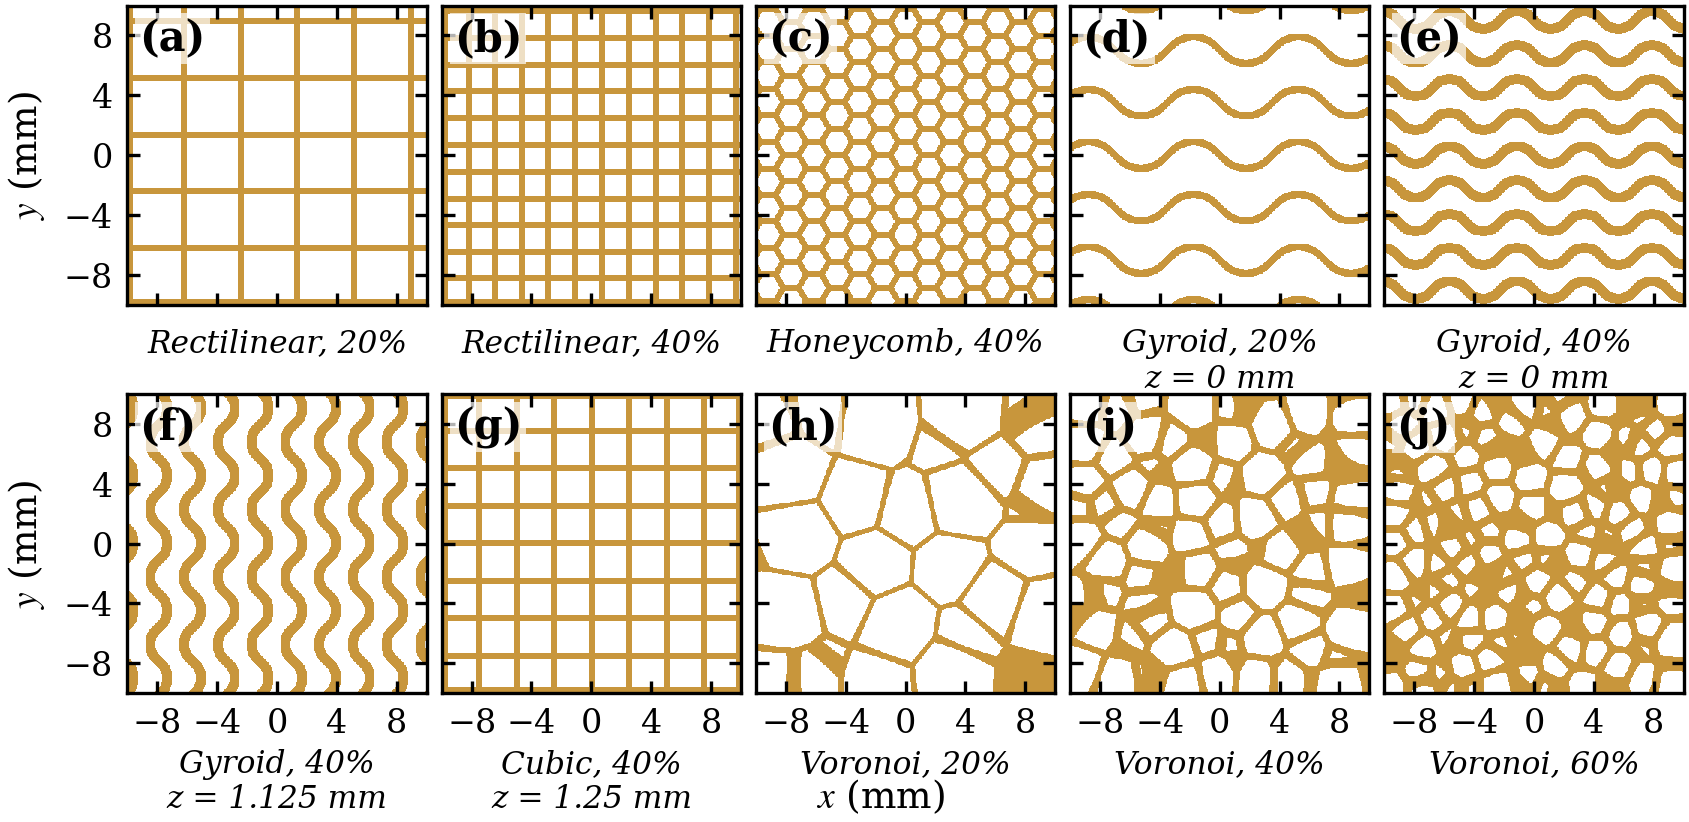
\includegraphics[width=\textwidth]{figure_1_geometry_cross_sections.png}
\caption{XY cross-sections of the five lattice geometries at representative infill levels, as implemented in the Geant4 simulation.  PLA is shown in colour; air gaps are white.  (a,b)~Rectilinear at 20\% and 40\%; (c)~honeycomb at 40\%; (d--f)~gyroid at 20\%, 40\%, and 40\% at a different $z$-slice showing the triply periodic structure.  The beam enters the page along~$+z$.}
\label{fig:geometries}
\end{figure*}

\paragraph{Rectilinear.}  Constructed using CSG (constructive solid geometry) with \texttt{G4Box} wall slabs.  Orthogonal X-wall and Y-wall families span the full sample depth ($\SI{10}{mm}$ along~$z$).  Truly binary path-length distribution: each particle crosses either full PLA walls or pure air gaps.  Cell sizes: 3.79/1.78/1.09/$\SI{0.72}{mm}$ at 20/40/60/80\%.

\paragraph{Honeycomb.}  Voxelised at $\SI{0.1}{mm}$ pixel resolution as columns extending the full depth along~$z$.  Hexagonal wall pattern with three edge families at $0^\circ/60^\circ/120^\circ$, creating Y-junctions at vertices.  The hex cell diameter~$d$ was determined by bisection (25 iterations) to match the beam-weighted infill fraction.  Binary path-length distribution.  Cell diameters: 3.81/1.77/1.09/$\SI{0.72}{mm}$ at 20/40/60/80\%.

\paragraph{Gyroid.}  Voxelised triply periodic minimal surface (TPMS) using the implicit level-set equation $F(\mathbf{r})=\sin(kx)\cos(ky)+\sin(ky)\cos(kz)+\sin(kz)\cos(kx)$.  Voxels with $|F|<t_{\mathrm{threshold}}$ were filled with PLA.  The threshold~$t$ and cell size were jointly tuned to match the target infill.  Continuous path-length distribution.  Cell sizes: 7.0/4.5/3.0/$\SI{2.0}{mm}$; thresholds: 0.305/0.617/0.914/1.197 at 20/40/60/80\%.

\paragraph{3D Grid (Cubic).}  CSG construction with three orthogonal wall families (X, Y, Z planes via \texttt{G4Box}).  Creates a true 3D lattice; some particles traverse walls in all three orientations.  Ternary path distribution ($\ell = 0$, partial, or full).  Cell sizes: 5.81/2.50/1.53/$\SI{0.95}{mm}$ at 20/40/60/80\%.

\paragraph{Voronoi.}  Voxelised centroidal Voronoi tessellation (CVT).  Seeds placed randomly in the sample volume and refined by 5 iterations of Lloyd relaxation (10\,000 probe points per iteration).  A point was classified as PLA if the distance difference to its two nearest Voronoi seeds fell below a wall thickness threshold, tuned by bisection (20 iterations, 20\,000 beam-weighted probes) to match the target infill.  Continuous, random path-length distribution.  Cell sizes: 4.0/2.5/1.8/$\SI{1.2}{mm}$; wall thresholds: 0.305/0.395/0.446/$\SI{0.441}{mm}$ at 20/40/60/80\%.

\subsection{Ray-trace validation}
\label{sec:raytrace}

An independent Monte Carlo ray-tracer computed the beam-weighted path-length distribution $p(\ell)$ for all 20 lattice configurations using $10^6$ straight-line rays per configuration, sampling from the same Gaussian beam profile ($\sigma=\SI{5}{mm}$).  For each ray at transverse position $(x,y)$, the PLA path length was computed by integrating the material indicator function along~$z$ through the $\SI{10}{mm}$ sample.  The geometric kurtosis
\begin{equation}
  \kappa_{\mathrm{geo}} = \frac{3\,\mathrm{Var}(\sigma^2)}{\mathrm{E}[\sigma^2]^2}
  \label{eq:kgeo_raytrace}
\end{equation}
was computed from the Highland-weighted variance of the path-length distribution.

For binary geometries (rectilinear, honeycomb), the ray-trace $\kappa_{\mathrm{geo}}$ agrees with the analytic formula $3(1-f)/f$ to sub-percent accuracy ($<1\%$), confirming the binary nature of the path-length distribution.  For continuous geometries (gyroid, 3D grid, Voronoi), the ray-trace provides the only available geometric prediction, as the path-length distribution is non-trivial.  Table~\ref{tab:raytrace} presents the complete ray-trace results.

\subsection{Analysis methodology}
\label{sec:analysis}

The excess kurtosis was estimated using the bias-corrected Fisher $g_2$ estimator (\texttt{scipy.stats.kurtosis} with \texttt{fisher=True, bias=False}), equivalent to the standard $k$-statistic.  For each configuration, the kurtosis of $\theta_x$ and $\theta_y$ were computed independently and averaged: $\kappa = (\kappa_x+\kappa_y)/2$.  Uncertainties were computed by bootstrap resampling (1\,000 resamples), with the standard deviation of the bootstrap distribution reported as $\mathrm{SE}(\kappa)$.  An analytical cross-check $\mathrm{SE}=\sqrt{24/N}$ was also computed.

The following quality cuts were applied to the projected scattering angle $\theta_x = \theta_{x,\mathrm{exit}} - \theta_{x,\mathrm{entry}}$:
\begin{itemize}
  \item \textbf{Energy cut:} exit energy $> 90\%$ of beam energy (removes hard bremsstrahlung events).
  \item \textbf{Angle cut:} $|\theta_x| < 10\,\sigma_{\mathrm{Highland}}(\text{solid})$ at the corresponding beam energy, using the solid control width for \emph{all} configurations (prevents topology-dependent bias).
  \item \textbf{Fiducial cut (primary):} $|\mathrm{entry}_x|<\SI{5}{mm}$, $|\mathrm{entry}_y|<\SI{10}{mm}$, matching the MIMOSA-26 sensor acceptance at the DESY~II test beam facility.
\end{itemize}
Full-acceptance results were provided as a cross-check; the fiducial cut is the primary result throughout.  Typical post-cut sample sizes ranged from 30\,000--47\,000 events per configuration (standard) to 127\,000--175\,000 (Voronoi).

%% ====================================================================
\section{Results}
\label{sec:results}
%% ====================================================================

\subsection{Angular distributions}
\label{sec:angular}

Figure~\ref{fig:angular} shows the projected scattering angle distributions for rectilinear geometry at $\SI{4}{GeV}$, comparing 20\%, 40\%, 60\%, 80\% infill and the solid PLA control, on a logarithmic vertical scale.  The core width (set by the Highland RMS) is similar across configurations, confirming that the Highland formula correctly predicts $\sigma$.  However, the tails diverge systematically: lower infill produces heavier tails.  At 20\% infill, the distribution develops a pronounced narrow core (from air-gap trajectories with minimal scattering) superimposed on broad tails (from wall-crossing trajectories that experience the full PLA scattering), the hallmark of a Gaussian mixture with high kurtosis.

\begin{figure}[t]
\centering
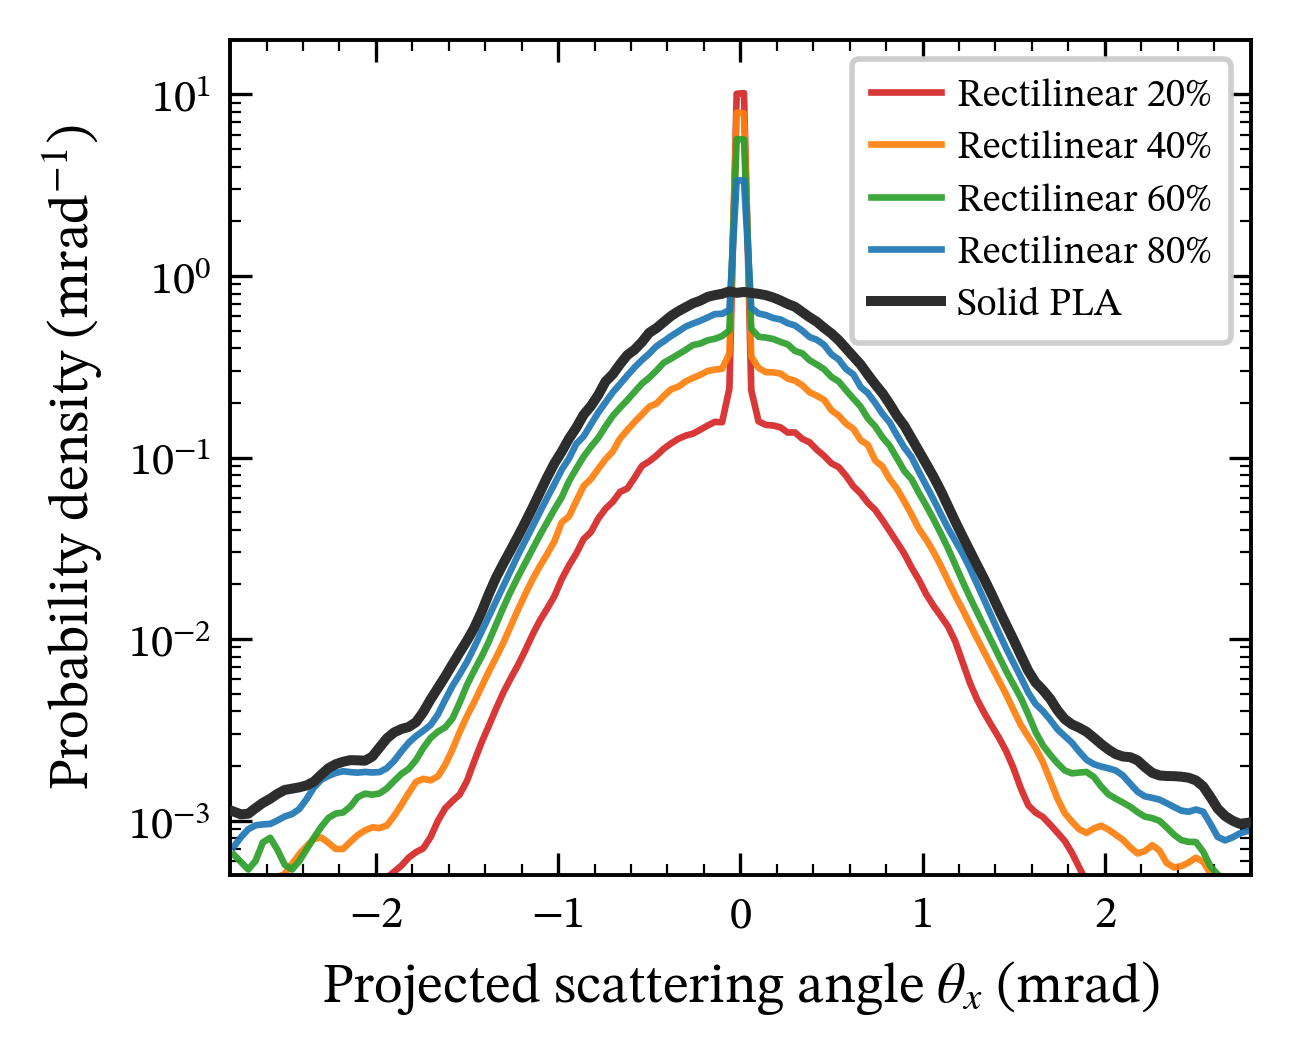
\includegraphics[width=\columnwidth]{figure_2_angular_distributions.png}
\caption{Projected scattering angle distributions $P(\theta_x)$ at $\SI{4}{GeV}$ for the rectilinear geometry at 20\%, 40\%, 60\%, 80\% infill (coloured curves) and the solid PLA control (black), plotted on a logarithmic vertical scale.  All distributions are normalised to unit area.  The core width is similar across configurations (Highland predicts $\sigma$ correctly), but the tails grow systematically with decreasing infill fraction.  The narrow central peak visible at 20\% infill arises from particles traversing only air gaps; the broad tails arise from particles crossing PLA walls.  The excess kurtosis increases from $\kappa=4.67\pm0.30$ at 80\% to $\kappa=16.05\pm0.41$ at 20\%, compared to $\kappa=3.62\pm0.26$ for the solid control.}
\label{fig:angular}
\end{figure}

\subsection{Solid control baselines}
\label{sec:controls}

Table~\ref{tab:results} presents the solid PLA control measurements.  The RMS scattering width $\sigma_x$ agrees with the Highland prediction to better than 1\% at all three energies ($\sigma_x/\sigma_H = 1.00$), confirming that the simulation correctly reproduces homogeneous-slab MCS.  The baseline excess kurtosis $\kappa_M$ ranges from 3.62 (4\,GeV) to 4.39 (2\,GeV), reflecting the energy-dependent Moli\`{e}re tail structure.  The Fr\"uhwirth--Liendl two-Gaussian analytical model ($w_2=0.02$, $r=3.2$)~\cite{FruhwirthRegler2001} predicts $\kappa_M = 3.57$, in good agreement with the Geant4 value at $\SI{4}{GeV}$.

\subsection{Infill scan at \texorpdfstring{$\SI{4}{GeV}$}{4 GeV}}
\label{sec:infill}

Table~\ref{tab:results} and Figure~\ref{fig:binary_vs_continuous} present the excess kurtosis for all 20 lattice configurations at $\SI{4}{GeV}$.  All five geometries show monotonically decreasing $\Delta\kappa = \kappa_{\mathrm{lattice}}-\kappa_{\mathrm{solid}}$ with increasing infill, as predicted by the mixture model (higher infill $\to$ more uniform paths $\to$ smaller variance $\to$ less kurtosis excess).  Binary lattices (rectilinear, honeycomb) produce the largest shifts ($\Delta\kappa\approx 5$ at 40\% infill, $\approx 12$ at 20\%), while continuous geometries (gyroid, Voronoi) show smaller shifts ($\Delta\kappa\approx 1.6$ at 40\%), consistent with their narrower path-length distributions.  The 3D grid falls between the two regimes ($\Delta\kappa\approx 3.0$ at 40\%), reflecting its ternary path distribution.

The rectilinear--honeycomb equivalence at matched infill ($\Delta\kappa = +5.03$ vs.\ $+4.98$ at 40\%) confirms that the excess kurtosis depends on the path-length distribution, not the specific wall topology.  Similarly, the gyroid--Voronoi similarity ($\Delta\kappa=+1.56$ vs.\ $+1.57$ at 40\%) reflects their shared property of continuous, smooth wall structures.

\begin{figure}[t]
\centering
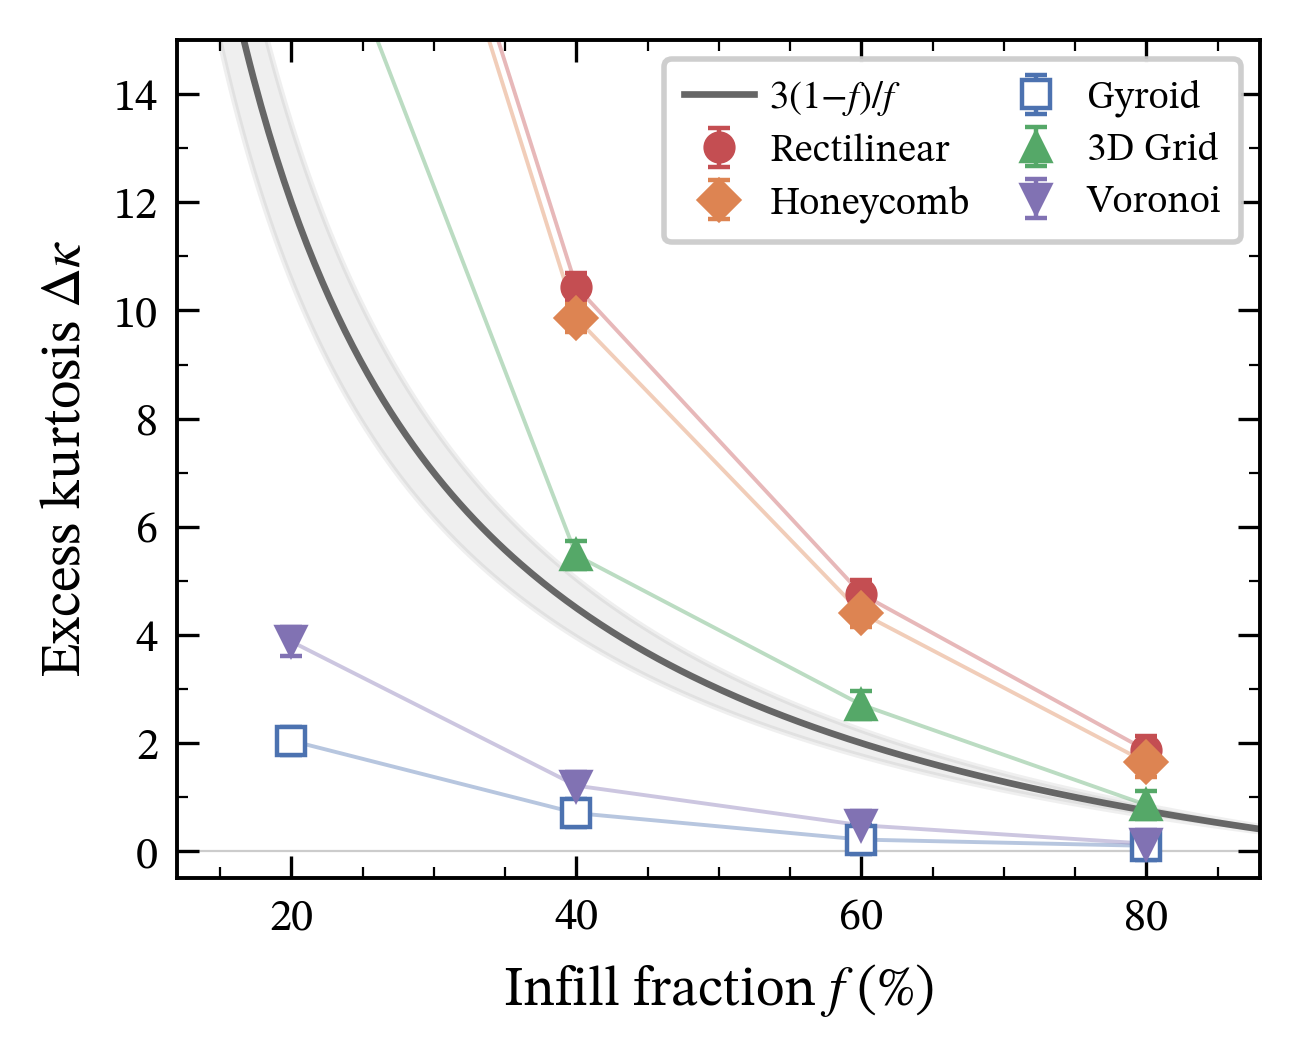
\includegraphics[width=\columnwidth]{figure_3_kurtosis_vs_infill.png}
\caption{Excess kurtosis $\Delta\kappa = \kappa_{\mathrm{lattice}}-\kappa_{\mathrm{solid}}$ versus infill fraction at $\SI{4}{GeV}$ for all five lattice geometries.  Filled circles: rectilinear; filled diamonds: honeycomb; open squares: gyroid; inverted open triangles: Voronoi; half-filled triangles: 3D grid.  The solid curve shows the binary-lattice analytic prediction $\kappa_{\mathrm{geo}}=3(1-f)/f$.  Error bars are bootstrap standard errors (1\,000 resamples).  Binary lattices closely track the $3(1-f)/f$ curve; continuous geometries lie systematically below, reflecting their narrower path-length distributions.}
\label{fig:binary_vs_continuous}
\end{figure}

\subsection{Universal equation validation}
\label{sec:validation}

Figure~\ref{fig:money} presents the central validation: measured excess kurtosis versus the prediction from the universal equation, Eq.~\eqref{eq:kappa_full}, for all 27 analysable configurations.  The predicted kurtosis uses $\kappa_M$ from the energy-matched solid control and $\kappa_{\mathrm{geo}}$ from the ray-trace (Table~\ref{tab:raytrace}).

\begin{figure}[t]
\centering
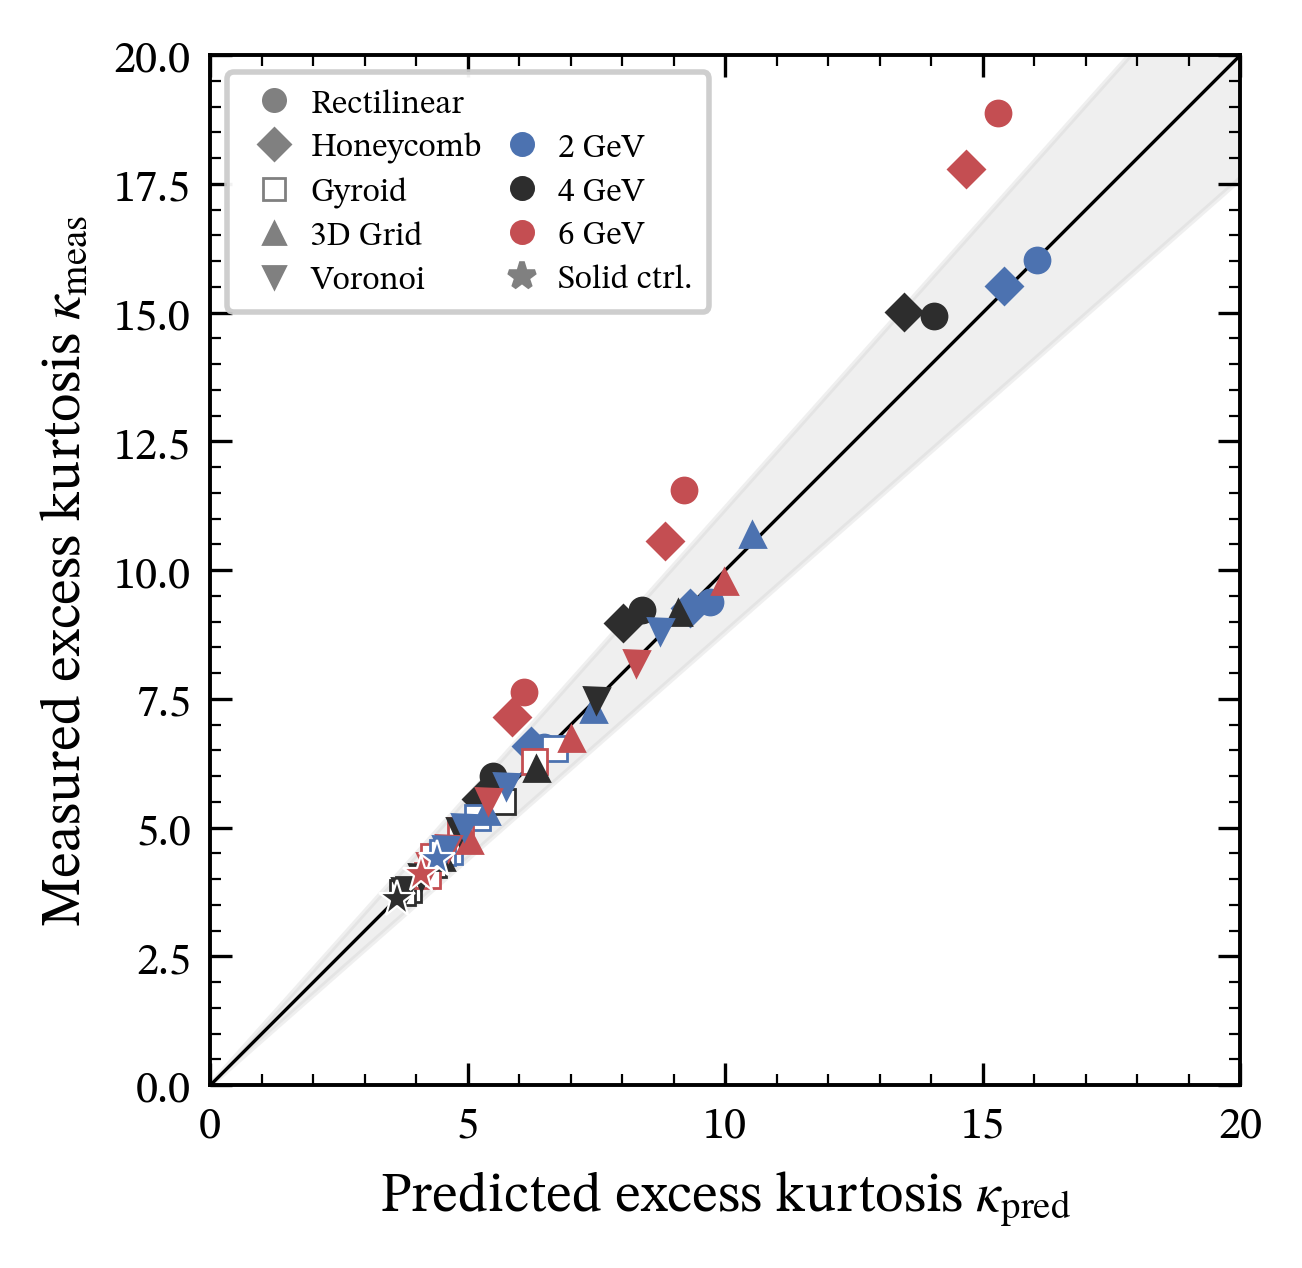
\includegraphics[width=\columnwidth]{figure_4_measured_vs_predicted.png}
\caption{Measured versus predicted excess kurtosis for all 27 analysable configurations.  The diagonal line represents perfect agreement.  Filled circles: rectilinear; filled diamonds: honeycomb (both binary); open squares: gyroid; inverted open triangles: Voronoi (both continuous); half-filled triangles: 3D grid (ternary).  Colours distinguish beam energies (blue: $\SI{2}{GeV}$; black: $\SI{4}{GeV}$; red: $\SI{6}{GeV}$).  Solid controls sit on the diagonal by construction ($\kappa_{\mathrm{pred}}=\kappa_M$).  The shaded band indicates a $\pm 12\%$ systematic deviation around the diagonal.  The universal equation captures the qualitative trends across all five geometries, four fill fractions, and three beam energies.  The systematic over-prediction for high-$\kappa_{\mathrm{geo}}$ binary configurations is attributed to the thin-wall Moli\`{e}re enhancement discussed in Section~\ref{sec:thinwall}.}
\label{fig:money}
\end{figure}

For continuous geometries with small $\kappa_{\mathrm{geo}}$ (gyroid, Voronoi at high infill), the equation provides accurate predictions; these configurations are dominated by the $\kappa_M$ baseline.  For binary lattices at low infill (large $\kappa_{\mathrm{geo}}$), the equation systematically over-predicts the measured kurtosis.  This discrepancy is attributed to the thin-wall Moli\`{e}re enhancement, discussed in Section~\ref{sec:thinwall}.

\subsection{Thin-wall Moli\`{e}re enhancement}
\label{sec:thinwall}

Figure~\ref{fig:thinwall} and Table~\ref{tab:results} quantify the systematic deviation for binary lattices.  The universal equation uses $\kappa_M$ extracted from the $\SI{10}{mm}$ solid PLA slab ($\ell/X_0\approx 0.032$).  In binary lattices, however, the scattering occurs in thin walls ($\sim\SI{0.4}{mm}$, $\ell/X_0\approx 0.001$).  At this much smaller thickness, the Moli\`{e}re screening parameter $\Omega_0\propto\ell$ is reduced by a factor of~$\sim 25$, and the single-scatter tail structure differs from that of the full slab.  The effective conditional kurtosis $\kappa_M^{\mathrm{(thin)}}$ for thin walls is not equal to the solid-slab value.

The thin-wall enhancement ratio, defined as $\Delta\kappa_{\mathrm{measured}}/\kappa_{\mathrm{geo}}$ (comparing the measured geometric excess to the pure Gaussian-mixture prediction), is energy-dependent: 1.00 at $\SI{2}{GeV}$, $1.10\pm0.11$ at $\SI{4}{GeV}$, and 1.22 at $\SI{6}{GeV}$.  The enhancement vanishes at low energy (where the scattering distribution is broadest and the single-scatter tails are relatively suppressed) and grows at higher energies where single-scattering tails become relatively more prominent.  A $\pm 12\%$ systematic uncertainty band on binary-lattice predictions is adopted for experimental applications.

\begin{figure}[t]
\centering
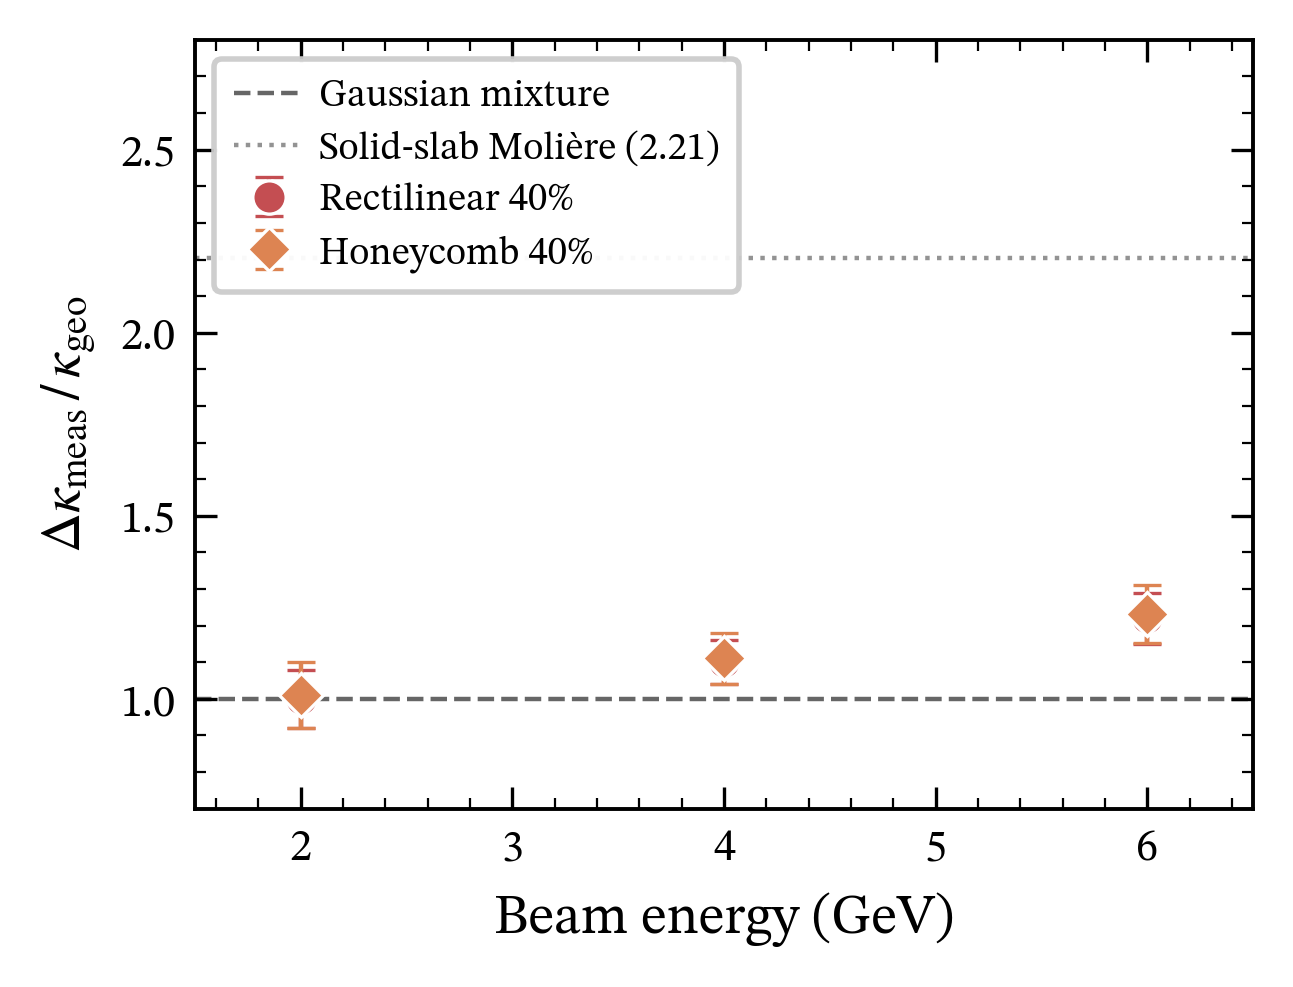
\includegraphics[width=\columnwidth]{figure_5_thin_wall_enhancement.png}
\caption{Thin-wall Moli\`{e}re enhancement ratio $\Delta\kappa_{\mathrm{measured}}/\kappa_{\mathrm{geo}}$ versus beam energy for binary lattices (rectilinear and honeycomb at 40\% infill).  The dashed horizontal line at 1.0 represents the pure Gaussian-mixture prediction ($\kappa_M=0$).  The enhancement vanishes at $\SI{2}{GeV}$ (ratio $\approx 1.00$) and grows to $\approx 1.22$ at $\SI{6}{GeV}$.  The theoretical Moli\`{e}re amplification factor $(1+\kappa_M/3)$ from the solid slab is shown for comparison (dotted line; $\approx 2.2$), demonstrating that the thin-wall conditional kurtosis is substantially smaller than the solid-slab value.  Error bars combine bootstrap and energy-scan statistical uncertainties.}
\label{fig:thinwall}
\end{figure}

\subsection{Energy dependence}
\label{sec:energy}

Table~\ref{tab:results} includes the energy-scan results for rectilinear 40\% and gyroid 40\% at 2, 4, and $\SI{6}{GeV}$.  For the rectilinear lattice, the total kurtosis decreases from 12.76 ($\SI{2}{GeV}$) to 8.43 ($\SI{6}{GeV}$), while the geometric excess $\Delta\kappa=\kappa_{\mathrm{lattice}}-\kappa_{\mathrm{solid}}(E)$ evolves from $+8.37$ to $+4.33$.  For the gyroid, $\Delta\kappa$ increases from $+0.01$ ($\SI{2}{GeV}$, indistinguishable from solid) to $+1.46$ ($\SI{6}{GeV}$).  The gyroid result at $\SI{2}{GeV}$ ($\kappa=4.40$ vs.\ $\kappa_{\mathrm{solid}}=4.39$) illustrates that at low energies the large Moli\`{e}re tails can mask the relatively small geometric contribution of continuous geometries.

\subsection{The \texorpdfstring{$1/N$}{1/N} convergence}
\label{sec:Nresults}

Figure~\ref{fig:Nscaling} validates the $1/N$ scaling of the geometric kurtosis.  Stacked rectilinear layers at 20\% infill with independent random phase shifts were simulated via ray-tracing for $N=1,2,4,10,20,100$.  Independent gyroid periods were simulated for $N=1,2,4,8,16$.

\begin{figure*}[t]
\centering
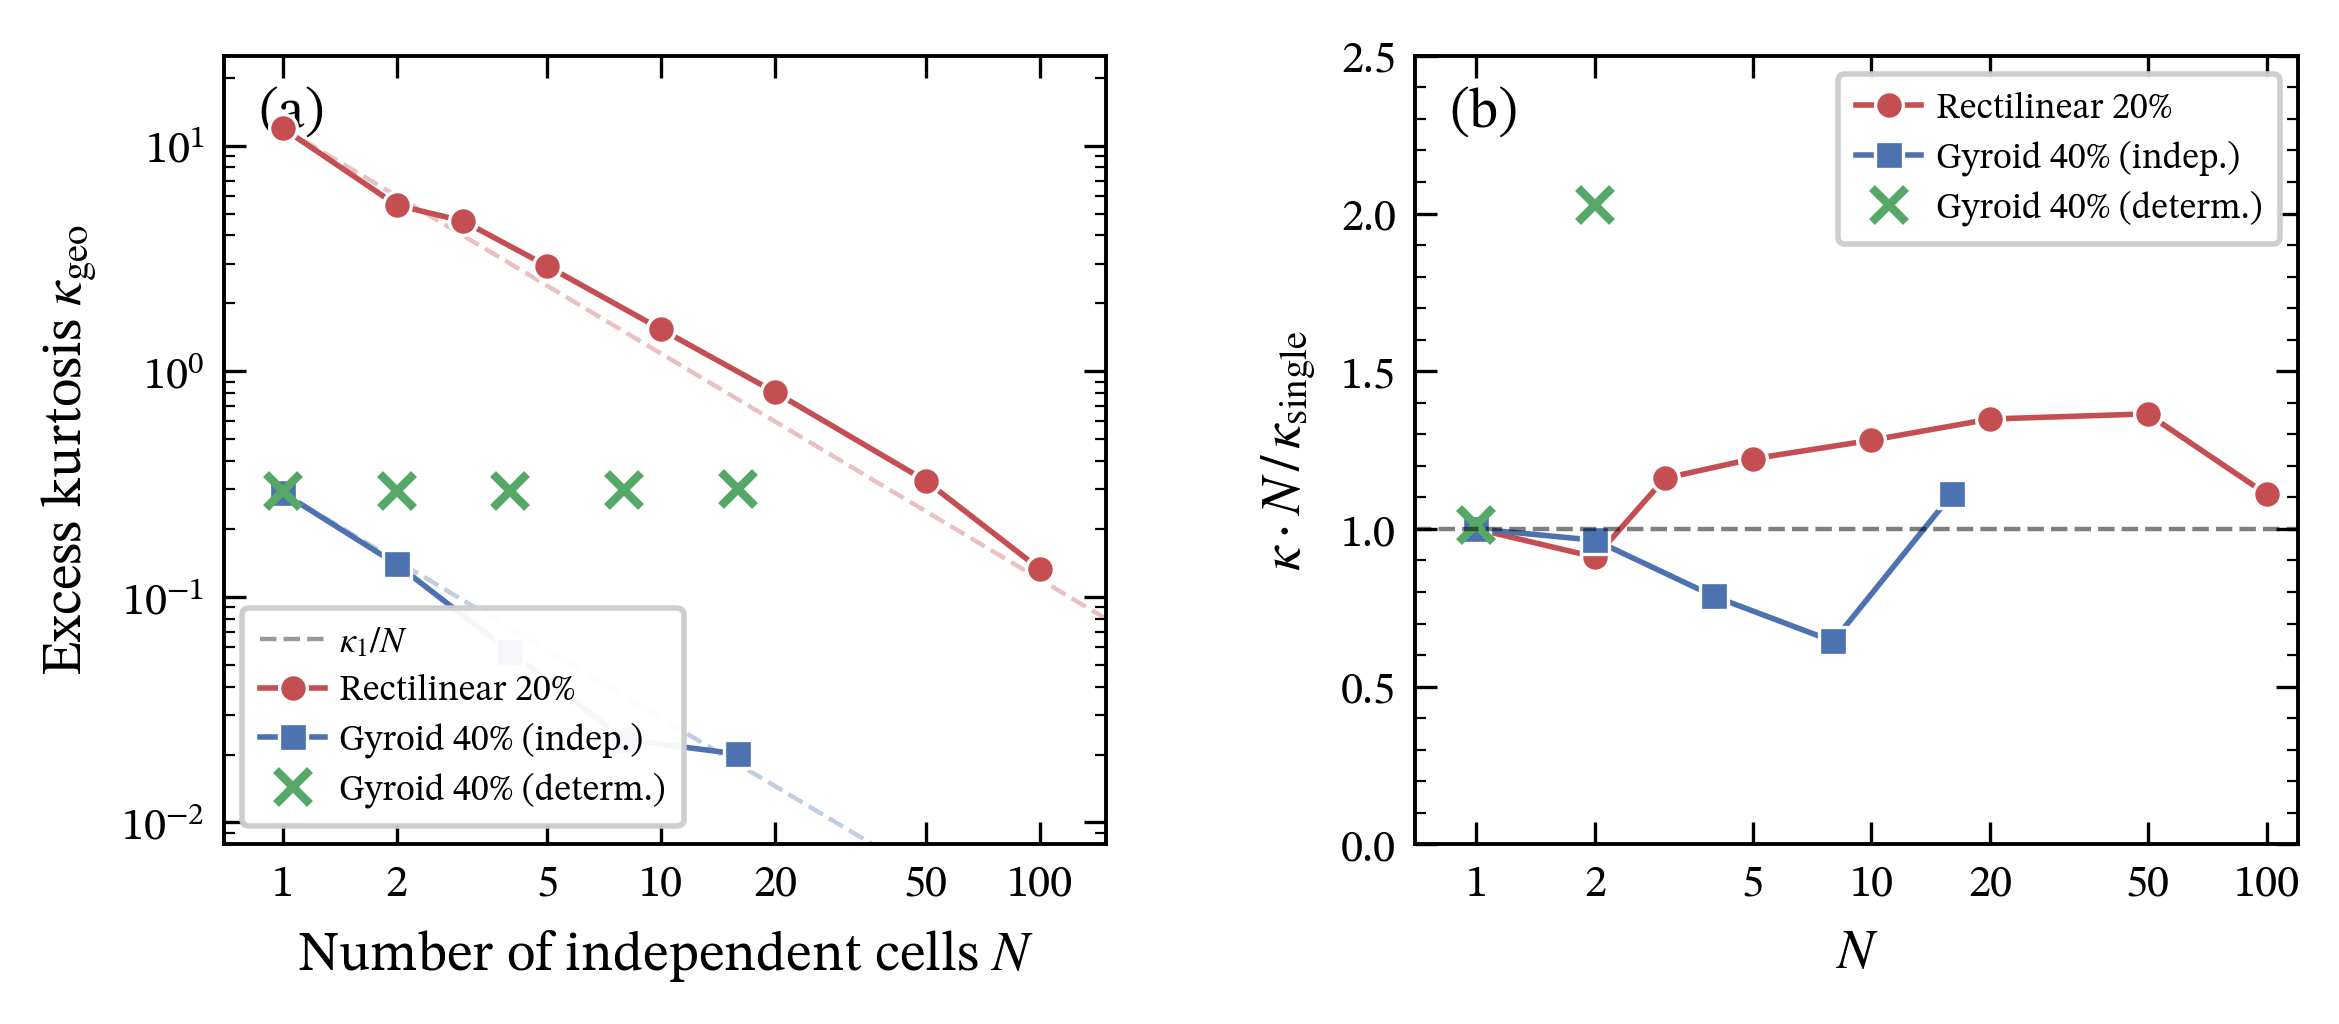
\includegraphics[width=\textwidth]{figure_6_n_scaling.png}
\caption{The $1/N$ convergence of excess kurtosis.  \textbf{Left:} $\kappa$ versus $N$ on log--log axes.  Blue circles: stacked rectilinear 20\% with independent random phases.  Green diamonds: independent gyroid 40\% periods.  Red crosses: deterministic (correlated) gyroid periods, showing $\kappa\approx\text{const}$ as expected for correlated cells.  Dashed lines: $\kappa=\kappa_{\mathrm{single}}/N$ predictions.  Both independent geometries follow the $1/N$ power law over two decades.  \textbf{Right:} Universality collapse $\kappa\cdot N/\kappa_{\mathrm{single}}$ versus~$N$.  Points cluster around 1.0 for independent cells, confirming the $1/N$ scaling.  Rectilinear data: $\kappa=11.97$ ($N=1$), 5.45 ($N=2$), 3.39 ($N=4$), 1.53 ($N=10$), 0.81 ($N=20$), 0.133 ($N=100$).  Gyroid independent: $\kappa=0.290$ ($N=1$), 0.140 ($N=2$), 0.057 ($N=4$), 0.023 ($N=8$), 0.020 ($N=16$).}
\label{fig:Nscaling}
\end{figure*}

The stacked rectilinear data follow $\kappa\propto N^{-1}$ from $\kappa=11.97$ at $N=1$ to $\kappa=0.133$ at $N=100$, spanning nearly two decades.  The universality collapse ratio $\kappa\cdot N/\kappa_{\mathrm{single}}$ approaches 1.0 for independent layers (Table~\ref{tab:results}).  The deterministic (correlated) gyroid shows $\kappa\approx 0.29 =\text{const}$, confirming that correlated cells do not benefit from the $1/N$ averaging.

\subsection{Three-model comparison}
\label{sec:threemodel}

Figure~\ref{fig:threemodels} compares three descriptions of the angular distribution for rectilinear 40\% at $\SI{4}{GeV}$: (i) the full Geant4 simulation; (ii) the Gaussian mixture model $P(\theta)=(1-f)\,G_{\mathrm{air}}(\theta) + f\,G_{\mathrm{PLA}}(\theta)$; and (iii) the same-mass Highland single Gaussian (all particles see the average thickness $\bar{\ell}=f\ell_{\mathrm{strut}}$).  The Highland Gaussian misses the heavy tails entirely.  The mixture model captures the bimodal structure (narrow core plus broad tails) and reproduces the measured kurtosis.

\begin{figure}[t]
\centering
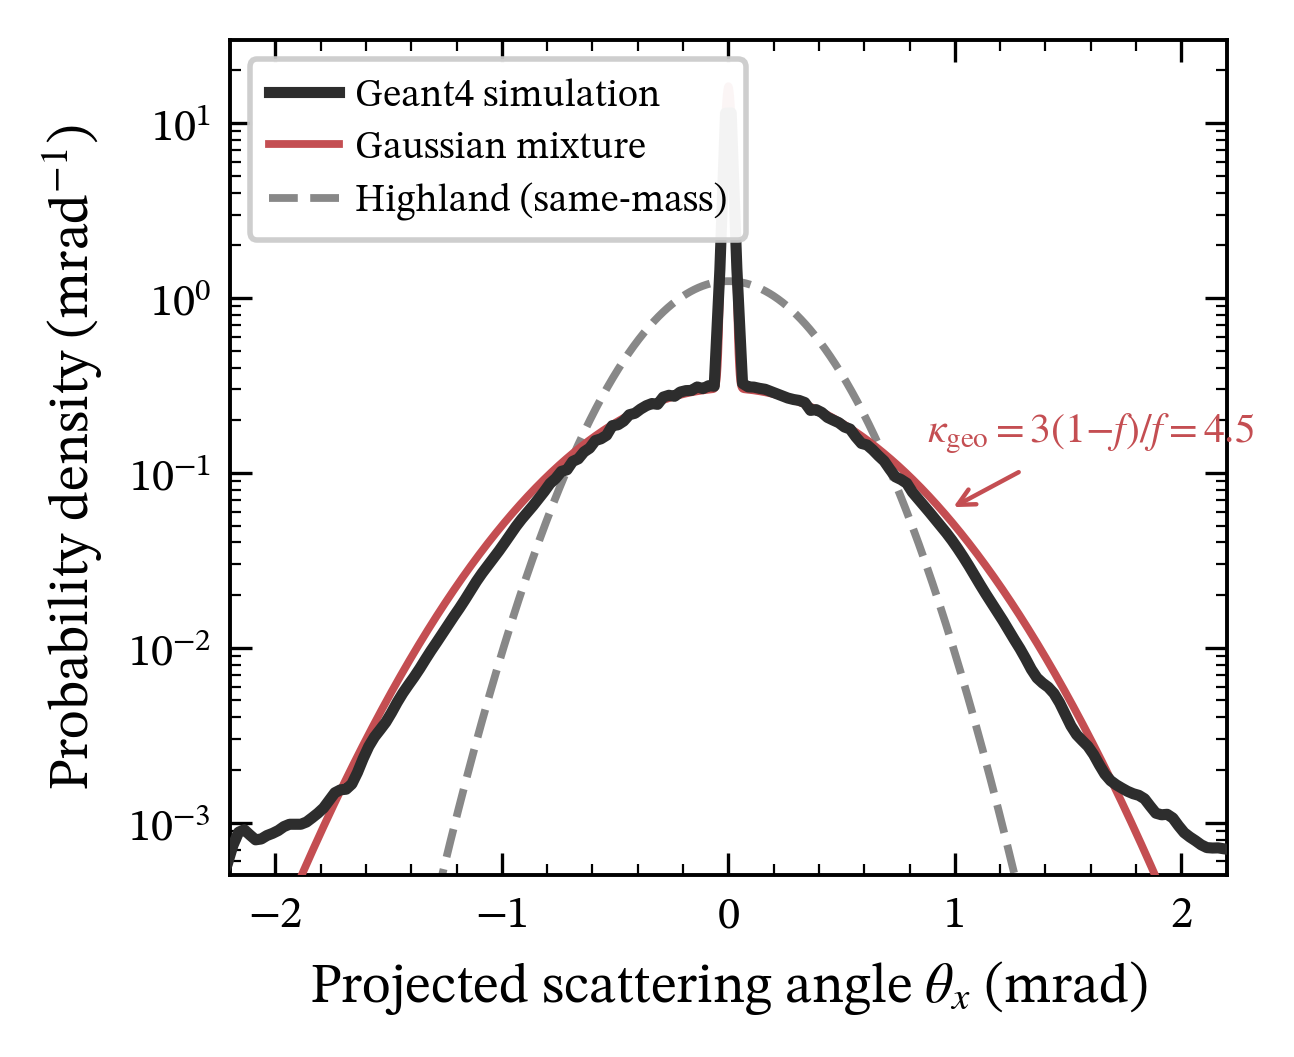
\includegraphics[width=\columnwidth]{figure_7_three_model_comparison.png}
\caption{Three-model comparison for rectilinear 40\% at $\SI{4}{GeV}$.  Black histogram: Geant4 simulation.  Red solid curve: Gaussian mixture model $P=(1-f)\,G_{\mathrm{air}}+f\,G_{\mathrm{PLA}}$, with component widths from the Highland formula.  Grey dashed curve: same-mass Highland single Gaussian (all particles traverse the average PLA thickness $\bar{\ell}=f\times\SI{10}{mm}=\SI{4}{mm}$).  The logarithmic vertical scale reveals that the Highland Gaussian under-predicts the tails by more than an order of magnitude at $|\theta_x|>3\sigma$, while the mixture model matches the simulation.  The geometric kurtosis $\kappa_{\mathrm{geo}}=3(1-f)/f = 4.5$ characterises the difference between the mixture and the single Gaussian.}
\label{fig:threemodels}
\end{figure}

%% --- COMPREHENSIVE RESULTS TABLE ---

\begin{table*}[t]
\centering
\caption{Complete simulation results for all 27 analysable configurations.  $N_{\mathrm{pass}}$: events after quality cuts.  $\sigma_x$: measured RMS projected scattering angle.  $\sigma_H$: Highland prediction for the average PLA thickness.  $\kappa$: measured excess kurtosis (bias-corrected Fisher $g_2$, average of $\theta_x$ and $\theta_y$).  SE: bootstrap standard error (1\,000 resamples).  $\Delta\kappa = \kappa_{\mathrm{lattice}}-\kappa_{\mathrm{solid}}(E)$: excess over energy-matched solid control.  All results use the fiducial acceptance ($|x_{\mathrm{entry}}|<\SI{5}{mm}$, $|y_{\mathrm{entry}}|<\SI{10}{mm}$).}
\label{tab:results}
\small
\resizebox{\textwidth}{!}{%
\begin{tabular}{llccrcccc}
\toprule
Geometry & Infill & Energy & $N_{\mathrm{pass}}$ & $\sigma_x$ & $\sigma_H$ & $\sigma_x/\sigma_H$ & $\kappa\pm\mathrm{SE}$ & $\Delta\kappa$ \\
         & (\%)   & (GeV)  &                     & (mrad)     & (mrad)     &                      &                        &                \\
\midrule
\multicolumn{9}{l}{\emph{Solid PLA controls}} \\
Solid    & 100 & 2 & 42\,826 & 1.05 & 1.05 & 1.00 & $4.39\pm0.32$ & --- \\
Solid    & 100 & 4 & 46\,102 & 0.53 & 0.53 & 1.00 & $3.62\pm0.26$ & --- \\
Solid    & 100 & 6 & 46\,881 & 0.35 & 0.35 & 1.00 & $4.10\pm0.31$ & --- \\
\midrule
\multicolumn{9}{l}{\emph{Lattice geometries at $\SI{4}{GeV}$}} \\
Rectilinear & 20 & 4 & 32\,039 & --- & --- & --- & $16.05\pm0.41$ & $+12.4$ \\
Rectilinear & 40 & 4 & 40\,587 & --- & --- & --- & $8.65\pm0.32$  & $+5.03$ \\
Rectilinear & 60 & 4 & 43\,927 & --- & --- & --- & $6.88\pm0.36$  & $+3.27$ \\
Rectilinear & 80 & 4 & 45\,329 & --- & --- & --- & $4.67\pm0.30$  & $+1.06$ \\
Honeycomb   & 20 & 4 & 33\,188 & --- & --- & --- & $15.32\pm0.35$ & $+11.7$ \\
Honeycomb   & 40 & 4 & 41\,735 & --- & --- & --- & $8.59\pm0.28$  & $+4.98$ \\
Honeycomb   & 60 & 4 & 44\,529 & --- & --- & --- & $5.58\pm0.25$  & $+1.96$ \\
Honeycomb   & 80 & 4 & 44\,893 & --- & --- & --- & $5.39\pm0.37$  & $+1.78$ \\
Gyroid      & 20 & 4 & 30\,218 & --- & --- & --- & $5.80\pm0.32$  & $+2.19$ \\
Gyroid      & 40 & 4 & 44\,197 & --- & --- & --- & $5.18\pm0.35$  & $+1.56$ \\
Gyroid      & 60 & 4 & 46\,002 & --- & --- & --- & $5.15\pm0.36$  & $+1.54$ \\
Gyroid      & 80 & 4 & 46\,324 & --- & --- & --- & $4.15\pm0.32$  & $+0.53$ \\
3D Grid     & 20 & 4 & 38\,104 & --- & --- & --- & $10.26\pm0.31$ & $+6.65$ \\
3D Grid     & 40 & 4 & 43\,660 & --- & --- & --- & $6.59\pm0.33$  & $+2.97$ \\
3D Grid     & 60 & 4 & 45\,463 & --- & --- & --- & $5.46\pm0.31$  & $+1.85$ \\
3D Grid     & 80 & 4 & 45\,902 & --- & --- & --- & $4.94\pm0.35$  & $+1.33$ \\
Voronoi     & 20 & 4 & 126\,841 & --- & --- & --- & $6.05\pm0.16$ & $+2.44$ \\
Voronoi     & 40 & 4 & 157\,230 & --- & --- & --- & $5.19\pm0.16$ & $+1.57$ \\
Voronoi     & 60 & 4 & 168\,927 & --- & --- & --- & $4.67\pm0.16$ & $+1.05$ \\
Voronoi     & 80 & 4 & 174\,558 & --- & --- & --- & $4.50\pm0.17$ & $+0.88$ \\
\midrule
\multicolumn{9}{l}{\emph{Energy scan at 40\% infill}} \\
Rectilinear & 40 & 2 & --- & 1.05 & --- & --- & $12.76$ & $+8.37$ \\
Rectilinear & 40 & 6 & --- & 0.35 & --- & --- & $8.43$  & $+4.33$ \\
Gyroid      & 40 & 2 & --- & 1.05 & --- & --- & $4.40$  & $+0.01$ \\
Gyroid      & 40 & 6 & --- & 0.35 & --- & --- & $5.56$  & $+1.46$ \\
\bottomrule
\end{tabular}%
}
\end{table*}

\begin{table*}[t]
\centering
\caption{Ray-trace geometric kurtosis $\kappa_{\mathrm{geo}}$ for all 20 lattice configurations.  $f_{\mathrm{hit}}$: beam-weighted fraction of rays intercepting PLA.  For binary geometries (rectilinear, honeycomb), the analytic formula $3(1-f)/f$ is shown and agrees with the ray-trace to $<1\%$.  For non-binary geometries, the analytic binary formula does not apply (marked N/A); the ray-trace provides the only geometric prediction.  $10^6$ rays per configuration.}
\label{tab:raytrace}
\small
\resizebox{\textwidth}{!}{%
\begin{tabular}{llcccc}
\toprule
Geometry & Infill (\%) & Cell size (mm) & $f_{\mathrm{hit}}$ & $\kappa_{\mathrm{geo}}$ (ray) & $3(1-f)/f$ (analytic) \\
\midrule
Rectilinear & 20 & 3.79 & 0.197 & 12.26 & 12.22 \\
Rectilinear & 40 & 1.78 & 0.388 & 4.73  & 4.73 \\
Rectilinear & 60 & 1.09 & 0.572 & 2.24  & 2.25 \\
Rectilinear & 80 & 0.72 & 0.739 & 1.06  & 1.06 \\
\midrule
Honeycomb   & 20 & 3.81 & 0.199 & 12.07 & 12.08 \\
Honeycomb   & 40 & 1.77 & 0.402 & 4.47  & 4.47 \\
Honeycomb   & 60 & 1.09 & 0.580 & 2.17  & 2.17 \\
Honeycomb   & 80 & 0.72 & 0.753 & 0.98  & 0.98 \\
\midrule
Gyroid      & 20 & 7.0  & 0.899 & 0.93  & N/A \\
Gyroid      & 40 & 4.5  & 0.965 & 0.32  & N/A \\
Gyroid      & 60 & 3.0  & 1.000 & 0.11  & N/A \\
Gyroid      & 80 & 2.0  & 1.000 & 0.03  & N/A \\
\midrule
3D Grid     & 20 & 5.81 & 1.000 & 8.67  & N/A \\
3D Grid     & 40 & 2.50 & 1.000 & 2.48  & N/A \\
3D Grid     & 60 & 1.58 & 1.000 & 0.93  & N/A \\
3D Grid     & 80 & 1.10 & 1.000 & 0.37  & N/A \\
\midrule
Voronoi     & 20 & 4.0  & 1.000 & 1.76  & N/A \\
Voronoi     & 40 & 2.5  & 1.000 & 0.55  & N/A \\
Voronoi     & 60 & 1.8  & 1.000 & 0.23  & N/A \\
Voronoi     & 80 & 1.2  & 1.000 & 0.09  & N/A \\
\bottomrule
\end{tabular}%
}
\end{table*}

%% ====================================================================
\section{Discussion}
\label{sec:discussion}
%% ====================================================================

\subsection{Implications for track fitting}
\label{sec:trackfitting}

A Kalman filter~\cite{Fruhwirth1987} models MCS process noise as Gaussian, assigning a single variance $\theta_0^2$ per material layer via the Highland formula.  The results presented here demonstrate that for structured detector modules, the scattering distribution has excess kurtosis $\kappa>0$, meaning the tails exceed the Gaussian prediction.  A Gaussian-Sum Filter (GSF)~\cite{FruhwirthRegler2001} models the process noise as a mixture of Gaussians, and the universal equation provides the mixture parameters directly from the module geometry.

For a typical silicon pixel module with active-area coverage $f\approx 0.93$, the geometric kurtosis is $\kappa_{\mathrm{geo}}\approx 3(1-0.93)/0.93 \approx 0.23$, and the total kurtosis is $\kappa\approx 3.6 + 0.23\times(1+3.6/3)\approx 4.1$.  The geometric contribution is small relative to the Moli\`{e}re baseline because the active coverage is high.

For a full barrel layer including inter-module gaps ($f\approx 0.7$), $\kappa_{\mathrm{geo}}\approx 3(1-0.7)/0.7\approx 1.3$, yielding $\kappa\approx 3.6 + 1.3\times 2.2\approx 6.5$.  The geometric contribution is now comparable to the Moli\`{e}re baseline, and a GSF would provide measurably better track-fit $\chi^2$ distributions~\cite{FruhwirthStrandlie2021}.

\subsection{Material budget characterisation}
\label{sec:matbudget}

The excess kurtosis contains structural information independent of the RMS scattering width.  While $\sigma_x$ measures the mean path length $\langle\ell\rangle$, $\kappa$ is sensitive to the \emph{variance} of the path-length distribution.  This complementarity means kurtosis could detect internal structural defects (e.g., printing defects in 3D-printed components) that leave the average material budget unchanged but modify the internal geometry.

The simulation results indicate that the gyroid offers the best match between idealised simulation and real 3D-printed (FDM) geometries, because both the simulation and the slicer use the same TPMS implicit-surface equation.  The rectilinear simulation provides an upper bound on $\Delta\kappa$ for real prints, because physical FDM printers alternate the layer direction, partially breaking the binary path-length distribution.

\subsection{The \texorpdfstring{$1/N$}{1/N} criterion for Gaussianity}
\label{sec:criterion}

The $1/N$ scaling provides a quantitative criterion for when the Highland Gaussian approximation is valid.  Requiring $\kappa_{\mathrm{geo}}<0.1$ at fill fraction $f=0.40$ ($\kappa_{\mathrm{geo,single}}=4.5$) gives $N > 45$ independent cells.  At $f=0.20$ ($\kappa_{\mathrm{geo,single}}=12.0$): $N>120$.  This explains why Highland works in bulk detectors---silicon sensors have $N\sim 10^5$ atomic layers---but fails in coarse lattices ($N\sim 1$--5 cells in a 3D-printed target with $\sim\SI{2}{mm}$ cell pitch across $\SI{10}{mm}$ depth).

\subsection{Broader applications}
\label{sec:broader}

The Gaussian scale mixture framework and the universal kurtosis equation are not limited to 3D-printed targets.  In muon tomography, cosmic-ray muons scatter through heterogeneous cargo containing varying densities and radiation lengths.  Non-Gaussian tails from the path-length variance improve the discrimination between threat and benign materials.  A reconstruction algorithm informed by Eq.~\eqref{eq:kappa_full} and the Gaussian scale mixture model of Wang et al.~\cite{Wang2009} could improve image quality by correctly modelling the heavy tails instead of clipping them.

In proton and ion therapy, the scattering-power formalism of Gottschalk~\cite{Gottschalk2010} assumes Gaussian angular distributions.  Patients' inhomogeneous anatomy (bone, soft tissue, air cavities) produces non-Gaussian scattering tails that could be predicted by the universal equation applied to the treatment-planning CT image.  Quantifying these tails may improve the accuracy of pencil-beam dose calculations in heterogeneous regions.  These applications are the subject of forthcoming work.

%% ====================================================================
\section{Conclusion}
\label{sec:conclusion}
%% ====================================================================

A closed-form expression for the excess kurtosis of the projected scattering angle distribution in heterogeneous media has been derived:
\begin{equation}
  \kappa = \kappa_M + \kappa_{\mathrm{geo}}\!\left(1+\frac{\kappa_M}{3}\right),
  \label{eq:conclusion}
\end{equation}
where $\kappa_M$ is the Moli\`{e}re kurtosis of the denser material and $\kappa_{\mathrm{geo}} = 3\,\mathrm{Var}(\sigma^2)/\mathrm{E}[\sigma^2]^2$ encodes the geometry through the path-length distribution.  The equation has been validated against $8.1\times10^7$ Geant4-simulated electrons across 27 configurations spanning five lattice geometries (rectilinear, honeycomb, gyroid, cubic grid, and Voronoi), four fill fractions (20--80\%), and three beam energies (2--6\,GeV).

For binary lattices, the simplified form $\kappa = (3+\kappa_M)/f - 3$ is confirmed to $\sim$12\%, with the systematic attributable to the energy-dependent thin-wall Moli\`{e}re enhancement.  The $1/N$ scaling $\kappa(N) = \kappa_{\mathrm{single}}/N$ is verified over two decades in~$N$ for both binary and continuous geometries with independent cells.

The equation provides three capabilities not previously available:
\begin{enumerate}
  \item A quantitative prediction for when the Highland Gaussian approximation fails, via the $1/N$ criterion;
  \item Mixture parameters for improved track fitting via Gaussian-Sum Filters, derived directly from the module geometry;
  \item A new observable---excess kurtosis---for structural characterisation of detector components, sensitive to the variance of the internal path-length distribution.
\end{enumerate}

Experimental validation with 3D-printed PLA lattice targets is planned at the DESY~II test beam facility.

%% ====================================================================
\section*{Acknowledgements}
%% ====================================================================

The author thanks the Geant4 collaboration for maintaining the simulation toolkit used in this work.  Computing resources were provided locally.

\bibliographystyle{elsarticle-num}
\bibliography{references}

\end{document}